\documentclass{sig-alternate}
%\usepackage{graphicx}

\begin{document}

\title{Geo-Store: A Spatially-Aware SPARQL Evaluation Engine (Demo Paper)}

\numberofauthors{3}
\author{
% 1st. author
\alignauthor
Chih-Jye Wang\\
    \affaddr{Department of CSSE}\\
    \affaddr{Auburn University}\\
    \affaddr{Auburn, AL, USA}\\
    \email{wangchj@auburn.edu}
% 2nd. author
\alignauthor
Wei-Shinn Ku\\
    \affaddr{Department of CSSE}\\
    \affaddr{Auburn University}\\
    \affaddr{Auburn, AL, USA}\\
    \email{weishinn@auburn.edu}
\alignauthor
Haiquan Chen\\
    \affaddr{Department of Math and CS}\\
    \affaddr{Valdosta State University}\\
    \affaddr{Valdosta, GA, USA}\\
    \email{hachen@valdosta.edu}
}

\conferenceinfo{GIS'12,} {November 6-9, 2012. Redondo Beach, CA,
USA}\CopyrightYear{2012}

\maketitle

\begin{abstract}
Nowadays, how to utilize spatial data on the semantic web has
attracted more and more interests from researcher due to the
rapidly increasing applications on geographic information, e.g.,
location-based services (LBS). However, there are currently
limited solutions providing efficient management of spatial data
on the semantic web. In this demonstration, we present Geo-Store,
a novel spatially-aware data management system built on the
state-of-art RDF triple store. By the augmentation of the standard
SPARQL language with spatial query filters, Geo-Store is able to
process complex queries with common spatial constraints.  Those
spatial filters are further analyzed and evaluated based on the
Spatially-Aware Hashing (SAH). In SAH, spatial data are
pre-processed and encoded with their Hilbert values by using
space-filling curves, resulting in a higher query processing
efficiency than the existing triple store approaches, with no
compromise in accuracy. Our system can be accessed at
http://ilab.auburn.edu/geostore.
\end{abstract}


\category{H.2.8}{Database Management}{Database
Application}[spatial databases and GIS]

\terms{Algorithms and Experimentation}

\keywords{Location-based services, space-filling curves, the
Semantic Web}

\section{Introduction}

%One of the values of the Hypertext Transfer Protocol (HTTP) often known as the World
%Wide Web is that one document is linked to other documents and relevant information
%can be obtained through the links. Similarly, the semantic web is a relatively new
%field of research and a fledgling set of standards that attempts to create a web of
%linked data in standardized format to help machine readability and processing. The
%web and the semantic web are tightly woven due to that much of semantic data are
%existing data on the web migrated to the new format or obtained by annotating
%the existing web with semantic information .
%
%Much of the semantic web data describe geospatial information, such as location of
%places, and geospatial information system that access this information is able to
%perform
%
%---

Semantic web is a fledgling field of research and set of standards to create a web of machine readable and processable data. The strength of this linked data is that, like the existing web, each piece of information can be linked to other pieces of information each identified by a unique identifier. For example, John could publish his information in the Friend Of A Friend\footnote{http://www.foaf-project.org/} (FOAF) format that is easily readable by machines. John's information may contain his basic information such as name and birthday; in addition, his information may also contain links to his friends in FOAF format, as well as things he like, such as a movie, which could also be uniquely identified and precisely described in semantic format\cite{lee:semantic_web}. In this example, a semantic aware application that has the identifier of John could retrieve information such as ``find all the movies liked by friends of John."

Due to recent research effort and growth, much of the semantic data describe geospatial entities, such as location and geographic extend of objects. Geospatial information systems that access semantic data can make powerful inference based on spatial and non-spatial information from various source and not limited to data of only certain domains. For example, to find a location for a new fast food restaurant, a location planning software needs to find name and location of near by restaurants as well as other types of point of interest, such as schools and shopping malls, within 5 kilometers of radius of candidate locations. The application pulls information from various sources and determines the optimal location. Despite the growth of semantic web data, it is an ongoing research to best manage and query geospatial semantic data to support upcoming applications.

Resource Description Framework (RDF) is a framework for describing entities (also known as \emph{resources} in semantic jargon) in semantic web format. Each property of an entity is described as a triple (S, P, O) consisting a subject, which denotes the entity, a predicate, denoting a property of the entity, and an object, the value of the property. Object of a triple can be either a literal or the subject of another triple (or the identifier of an entity) creating a link between the entities. The linking between entities forms a graph. A system that manages and control access to a set of triple is often called a \emph{triple store}.

The purpose of this paper is to demonstrate Geo-Store~\cite{journals/internet/KuCWL}, a geospatial-enabled triple store. The system implements spatial query filters, which allow user to integrate spatial relationships into SPARQL queries. The system utilizes spatial-aware hashing to efficiently implement these spatial features. In addition, the system provides a query builder for the user to easily compose geospatial queries. Our system utilizes spatial aware indexing to facilitate efficient evaluation of spatial filters. The system is built on top of RDF-3X~\cite{DBLP:journals/vldb/NeumannW10}, a scalable RDF management system. 
\section{System Design}

Figure~\ref{fig:architect} shows the architecture of
Geo-Store~\cite{journals/internet/KuCWL}. The major components of
Geo-Store include a spatially-aware mapping module, an internal
indexing module~\cite{DBLP:journals/vldb/NeumannW10}, and a query
planner/analyzer module.

\begin{figure}
\centering
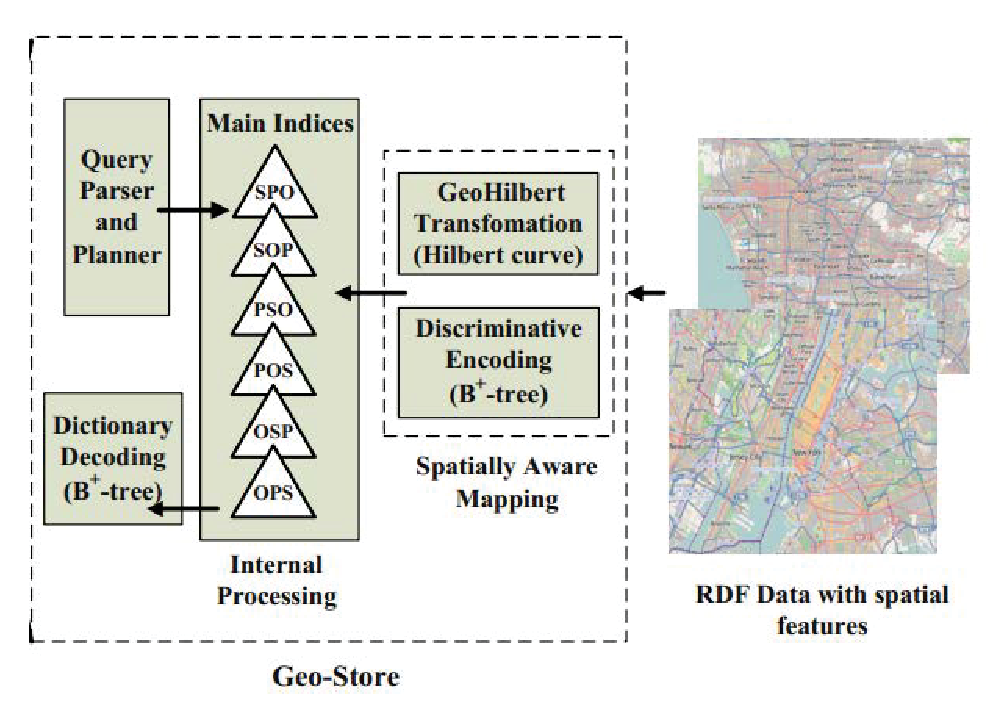
\includegraphics[width=3in]{images/architect.eps}
\caption{System Architecture of Geo-Store}\label{fig:architect}
\end{figure}

\subsection{The Spatially-Aware Hashing Module}

In order to support efficient spatial query processing, Geo-Store
employs Spatially-Aware Hashing (SAH), where Hilbert space filling
curves are generated and the Hilbert values (integers) of the
literals containing coordinates information (latitude/longitude)
are calculated and then appended to the original triple data
source as location indicators~\cite{journals/internet/KuCWL}.
Spatially-Aware Hashing provides the following advantages. First,
the Hilbert values of points of interest (POI) serves as
approximate location indicators. In other words, by only checking
with its Hilbert value, we can identify the small bounding grid (a
rectangular region) in which a specific POI resides. Second, those
location indicators perverse spatial locality, i.e., two POI's
that are geographically close are hashed into close integers at
most cases.  Third, the use of Hilbert values as location
indicators bases spatial query processing on integer number
comparison, reducing the occurrence of long string
(latitude/longitude) comparison, which is very costly in
computation and storage in triple stores.


\subsection{Spatial Query Analyzer}

In Geo-Store, spatial queries are expressed by using spatial query
filters and those filter are processed by our query analyzer.
When a query is submitted, the query analyzer looks for any
spatial filter in that query. If there is any spatial filter, the
analyzer uses the spatial-aware hashing to identify a list of
Hilbert values (serve as integer location indicators) that are
involved by the filter. Since the underlying triple store,
RDF-3X~\cite{DBLP:journals/vldb/NeumannW10}, are built on standard
SPARQL patterns without awareness of any spatial context, our
query analyzer then translates the related hash values into query
patterns and insert them as the patterns into the original query.
For multiple spatial query filters, the query analyzer applies
intersection operations to find the geographic locations
satisfying all the spatial constraints.

\section{Demonstration}

\subsection{Spatial Queries}

In Geo-Store, we implemented three basic spatial filters as
building blocks for constructing complex spatial queries.

\underline{\textbf{Window Filter}} \\
A window filter describes a binding of a query variable in a
SPARQL query to a specified rectangular region in a 2-dimensional
space.

\begin{verbatim}
SELECT ?name ?location WHERE{
    ?e <name> ?name.
    ?e <coordinates> ?location.
    within(?location, 32.5955, -85.4909, 32.6122,
           -85.4739)
}
\end{verbatim}
%\caption{\small Skyline SQL Clause.
%\label{fig:skyline_sql}}

\underline{\textbf{Range Filter}} \\
A range filter imposes a binding of a query variable in a SPARQL
query to a circular region in a 2-dimensional space, given a
center point and a radius.

\begin{verbatim}
SELECT ?name ?location WHERE{
    ?e <name> ?name.
    ?e <coordinates> ?location.
    within(?location, 32.597178, -85.463086, 1500)
}
\end{verbatim}

\underline{\textbf{Nearby Filter}} \\
A nearby filter can be used to issue a \emph{k}-NN query, given
the location of a query point and the \emph{k} value.

\begin{verbatim}
SELECT ?name ?location WHERE{
    ?e <name> ?name.
    ?e <coordinates> ?location.
    nearby(?location, 32.607985, -85.481439, 3)
}
\end{verbatim}

\subsection{Query Builder}

Figure~\ref{fig:geostore_web} shows the GUI of the query builder.
The GUI consists of two parts. The top part is the query editor
that allows the user to manually enter a SPARQL query with
aforementioned spatial query filters. The bottom part is the
interface that prompts the user to provide the corresponding query
parameters so that spatial filters can be generated automatically
and inserted into a standard SPARQL query incrementally. To
evaluate a SPARQL query with spatial constraints/patterns, the
spatial constraints are first dealt with by our spatial query
analyzer while the non-spatial constraints are submitted to the
underlying triple store
RDF-3X~\cite{DBLP:journals/vldb/NeumannW10} for execution.

\begin{figure}[t]
\centering
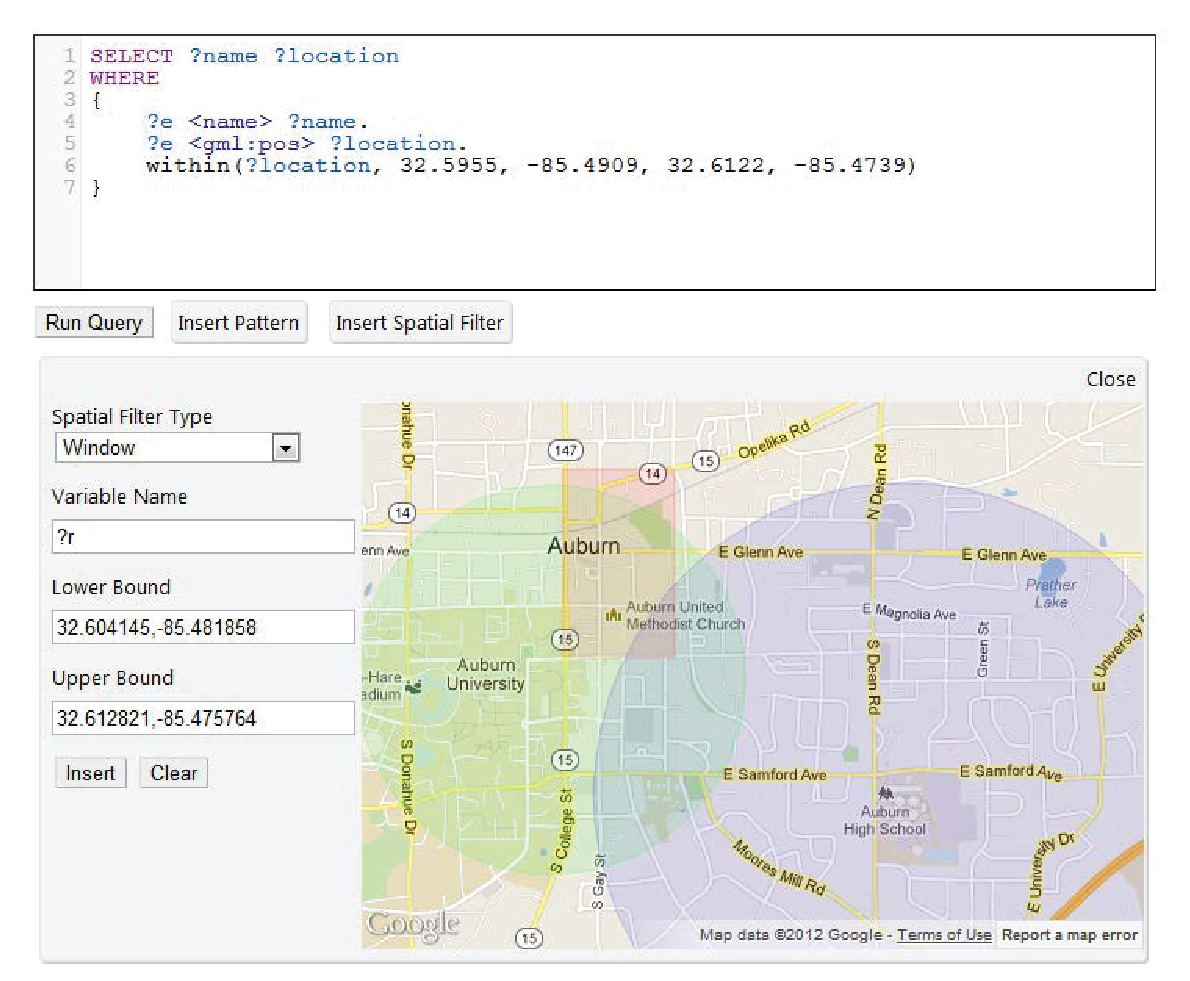
\includegraphics[width=3.3in]{images/geostore_web.eps}
\caption{Query Builder GUI of Geo-Store}\label{fig:geostore_web}
\end{figure}

\section{Conclusions}
Our system implements spatial query types in the form of SPARQL query filtesr. Currently, the filters types are window query, range (with and without binding), and nearby queries. The query analyzer uses the spatial-aware hashing index to facilitate the evaluation of spatial queries.

%ACKNOWLEDGMENTS are optional
%\section{Acknowledgments}
%This section is optional; it is a location for you
%to acknowledge grants, funding, editing assistance and
%what have you.  In the present case, for example, the
%authors would like to thank Gerald Murray of ACM for
%his help in codifying this \textit{Author's Guide}
%and the \textbf{.cls} and \textbf{.tex} files that it describes.

%\small
\bibliographystyle{abbrv}
\bibliography{gis2012}
\balancecolumns
\end{document}
